
%(BEGIN_QUESTION)
% Copyright 2008, Tony R. Kuphaldt, released under the Creative Commons Attribution License (v 1.0)
% This means you may do almost anything with this work of mine, so long as you give me proper credit

Calculate the current and all voltage drops in this loop-powered transmitter circuit, assuming the pressure transmitter is calibrated for a range of 0 to 70 PSI, 4 to 20 mADC.  Be sure to show all your work!

$$\includegraphics[width=15.5cm]{i03232x01.eps}$$

% No blank lines allowed between lines of an \halign structure!
% I use comments (%) instead, so that TeX doesn't choke.

$$\vbox{\offinterlineskip
\halign{\strut
\vrule \quad\hfil # \ \hfil & 
\vrule \quad\hfil # \ \hfil & 
\vrule \quad\hfil # \ \hfil & 
\vrule \quad\hfil # \ \hfil \vrule \cr
\noalign{\hrule}
%
% First row
Applied & Current & Transmitter & Resistor \cr
%
pressure (PSI) & (mA) & voltage (V) & voltage (V) \cr
%
\noalign{\hrule}
%
% Another row
0 PSI &  &  &  \cr
%
\noalign{\hrule}
%
% Another row
15 PSI &  &  &  \cr
%
\noalign{\hrule}
%
% Another row
20 PSI &  &  &  \cr
%
\noalign{\hrule}
%
% Another row
35 PSI &  &  &  \cr
%
\noalign{\hrule}
%
% Another row
60 PSI &  &  &  \cr
%
\noalign{\hrule}
%
% Another row
70 PSI &  &  &  \cr
%
\noalign{\hrule}
} % End of \halign 
}$$ % End of \vbox

\vfil 

\underbar{file i03232}
\eject
%(END_QUESTION)





%(BEGIN_ANSWER)

This is a graded question -- no answers or hints given!

%(END_ANSWER)





%(BEGIN_NOTES)

Current in this circuit is a simple linear function of applied pressure, according to the transmitter's calibrated range of 0 to 70 PSI.  Once we know the current in the circuit for each value of applied pressure, calculating resistor voltage drop is a simple matter of applying Ohm's Law.  Once we know the resistor voltage drop, the transmitter's voltage will be the difference between the resistor's drop and the supply voltage.

% No blank lines allowed between lines of an \halign structure!
% I use comments (%) instead, so that TeX doesn't choke.

$$\vbox{\offinterlineskip
\halign{\strut
\vrule \quad\hfil # \ \hfil & 
\vrule \quad\hfil # \ \hfil & 
\vrule \quad\hfil # \ \hfil & 
\vrule \quad\hfil # \ \hfil \vrule \cr
\noalign{\hrule}
%
% First row
Applied & Current & Transmitter & Resistor \cr
%
pressure (PSI) & (mA) & voltage (V) & voltage (V) \cr
%
\noalign{\hrule}
%
% Another row
0 PSI & 4 & 24 & 1 \cr
%
\noalign{\hrule}
%
% Another row
15 PSI & 7.429 & 23.143 & 1.857 \cr
%
\noalign{\hrule}
%
% Another row
20 PSI & 8.571 & 22.857 & 2.143 \cr
%
\noalign{\hrule}
%
% Another row
35 PSI & 12 & 22 & 3 \cr
%
\noalign{\hrule}
%
% Another row
60 PSI & 17.714 & 20.571 & 4.429 \cr
%
\noalign{\hrule}
%
% Another row
70 PSI & 20 & 20 & 5 \cr
%
\noalign{\hrule}
} % End of \halign 
}$$ % End of \vbox

%INDEX% Electronics review: 4-20 mA loop circuits

%(END_NOTES)


